\subsection{Audience behaviours in the collective decision-making process} \label{sect:listener_models}

\subsection*{Simple Listener Model}
Having addressed multiple ways for the speaker to construct an argument, it is imperative to define the strategies that listener agents may employ to update their attitudes. Drawing inspiration from the Friedkin and Johnsen model~\cite{Friedkin1999SocialChange}, we define an update rule that maintains an element of the agents previous beliefs as well as assimilating the new information. 

The equation we will use shall be


\lhead{\textit{Listener Models}}
\begin{equation} \label{eq:BU_update_rule}
    \mathbf{P}^{t+1}_L = \alpha \cdot \mathbf{P}^{t}_L + (1 - \alpha) \cdot  \frac{\mathbf{A} \odot \mathbf{P}^t_L}{\mathbf{A} \cdot \mathbf{P}^t_L}
\end{equation}

where $\alpha$ is a parameter on the interval $[0, 1]$ that governs the susceptibility of an agent to new information~\cite{Hegselmann2002Opinion}. In Hegselmann's work this parameter differs depending upon how reliable the listener believes the other agent to be, while, here, it is constant across all agents. Finally, $\odot$ denotes the elementwise or Haramaard product~\cite{Johnson1990MatrixApplications}. The last component of this equation serves to condition the speaker's argument $\mathbf{A}$  on the listener's original beliefs and then renormalise this such that the agent's probability distribution remains valid by summing to $1$. Any agent whose set of beliefs loses this property is described as incoherent and withdrawn from the population~\cite{Lee2018CombiningConsensus}. Furthermore, it is important to manage the listeners use of this update equation as, in the case where the cardinality of the set $\mathbf{A}$, $|\mathbf{A}| = 0$ \cref{eq:BU_update_rule} is undefined. In this case, the listener simply will not update.  

It should be noted that the Open Model represents a special case. The above equation is tailored toward arguments of binary vectors so if the Open Model is applied the equation becomes 

\begin{equation} 
    \mathbf{P}^{t+1}_L = \alpha \cdot \mathbf{P}^{t}_L + (1 - \alpha) \cdot \mathbf{A} 
\end{equation}


\subsection*{Discerning Model}

The previous model deprives the listener agent of the ability to disregard any information it receives; it will always update its beliefs based on new information. In order to address this, the model requires that when the listener reverses the process used to create the argument on its own beliefs, the same condition must be met. This is only possible in the Bottom Up and Top Down models as they involve a specified criterion that the argument must meet to be transmitted. Consider the following example for illustration. 

Let the speaker broadcast \hspace{10em}

\begin{minipage}[ht]{0.45\textwidth}
\begin{center}
$\mathbf{A} = \begin{bmatrix}
    1\\
    0\\
    1
\end{bmatrix}$
\end{center}
\end{minipage}
and let
\begin{minipage}[ht]{0.45\textwidth} 
$P^t_L = \begin{bmatrix}
    0.6\\
    0.15\\
    0.25
\end{bmatrix}$
\end{minipage}

In the case that this argument is constructed with the Bottom Up method with a threshold $\gamma = 0.4$, the listener compares the argument with its own beliefs. It finds that $p_1 > \gamma$ passing the requirement, $p_2$ is not asserted so is not considered, and finally $p_3 < \gamma$. Since the assertion of $H_3$ seems unlikely to the agent, it rejects the assertion outright, refusing to update. Similarly, if the argument is created with the Top Down model with a threshold $\gamma = 0.8$, then the listener takes the dot product of $\mathbf{A}$ and $P_L^t$. In this case this returns a value of $0.85$ which is greater than $\gamma$ so the listener accepts the argument and updates accordingly. 


\subsection*{Spiteful Model}

The previous model is relatively passive in the sense that, should it disagree with the argument, it does not update its beliefs whatsoever. However, anyone who has ever been told to ``calm down'' while irate can likely attest that occasionally an argument can often backfire if the listener finds it incredible. In this model, the criteria for disagreeing with an argument are as above, but, instead of passively ignoring the assertion, the listener will update using $\mathbf{A}^c$.

It is expected that both the Discerning and Spiteful models will cause divisions in the population, creating regions in which agents are incapable of responding to an argument. 



\subsection*{Stubborn Model}

The final listener model aims to mimic the growth of stubbornness as time progresses. In this model, $\alpha$ from \cref{eq:BU_update_rule} is a function of the number of arguments the agent has received, henceforth given by $\tau$. The equation is

\begin{equation}
    \alpha = 1 - (1 - \alpha_0) e^{-\lambda \tau}
\end{equation}

where $\alpha_0$ is the initial value of $\alpha$ and $\lambda = \frac{K}{t_max}$ is a rate at which the agents become stubborn. This allows an agent to be strongly influenced by the early arguments it hears but then, as it hears more and more, come to rely more heavily on its previous beliefs. This can be seen in \cref{fig:stubbornness_curve}. 


\begin{figure}[H]
    \centering
    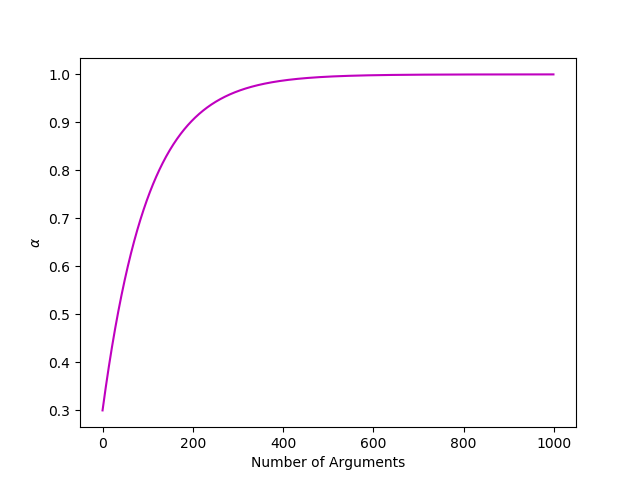
\includegraphics[width=0.49\textwidth]{Images/Misc/Stubbornness.png}
    \caption{A graph to show the rate at which agents change the importance they place on new information in the Stubborn Model. \textit{Using $\alpha_0 = 0.3, \lambda = 0.01$}}
    \label{fig:stubbornness_curve}
\end{figure}